\begin{refsection}[research/sato/group.bib]
\nocite{*}
\chapter{Programming Environment Research Team}

\section{Members}

\begin{itemize}
  \item[] Mitsuhisa Sato (Team Leader)
  \item[] Hitoshi Murai (Research Scientist)
  \item[] Miwako Tsuji (Research Scientist) 
  \item[] Masahiro Nakao (Research Scientist)
  \item[] Jinpil Lee (Postdoc Researcher)
  \item[] Yuetsu Kodama (Senior Research Scientist)
  \item[] Hidetoshi Iwashita (Research Associate)
  \item[] Shinichi Ito (Research Associate)
  \item[] Makoto Ishihara (Agency Staff)
  \item[] Masahiro Yasugi (Senior Visiting Researcher)
  \item[] Hitoshi Sakagami (Senior Visiting Researcher)
  \item[] Brian Wylie (Visiting Researcher)
  \item[] Christian Feld (Visiting Researcher)
  \item[] Kengo Nakajima (Senior Visiting Researcher)
  \item[] Tomoko Nakashima (Assistant)
\end{itemize}

\section{Research Activities}

The K computer system is a massively parallel system which has a huge
number of processors connected by the high-speed network. In order to
exploit full potential computing power to carry out advanced
computational science, efficient parallel programming is required to
coordinate these processors to perform scientific computing. We
conducts researches and developments on parallel programming models
and language to exploit full potentials of large-scale parallelism in
the K computer and increase productivity of parallel programming.

In 2015FY, in order to archive these objectives above, we carried out the following researches:

\begin{description}
\item[(1)] We are working on the development and improvement of XcalableMP (XMP) programming languages. XcalableMP is a directive-based language extension, designed by XcalableMP Specification Working Group (XMP Spec WG) including some members from our team as a community effort in Japan. It allows users to develop parallel programs for distributed memory systems easily and to tune the performance by having minimal and simple notations. In this year, we have improved Coarray functions in Fortran. The feature of coarray of the Omni XcalableMP compiler is implemented for the K compiler. In addition, some benchmarks and an application are parallelized with XcalableMP and their performance is evaluated on the K computer.

\item[(2)] As an extension of XcalableMP to exascale computing, we are proposing a new programming model, XcalableACC, for emerging accelerator clusters, by integrating XcalableMP and OpenACC. We continue working on the language design and the compiler development of XcalableACC. This research is funded by JST CREST project on “post-petascale computing”.

\item[(3)] Co-design for HPC is a bidirectional approach, where a system would be designed on demand from applications, and applications must be optimized to the system. We started the design of tools for co-design, including the SCAMP profiler for the network of large scale systems.

\item[(4)] As the post-K computer will be a large-scale multicore-based system, we are investigating programming models for manycore-based parallel systems as a next version of XcalableMP, including dynamic tasking and load balancing as well as advanced PGAS models for distributed memory systems.


\item[(5)] We conducted several collaborations on the performance evaluation with JSC, University of Tsukuba, Kyusyu Institute of Technology and other groups. In the collaborations with Kyusyu Institute of Technology, a task parallel language Tascell was evaluated on the K computer. We are developing tools for performance analysis of large-scale parallel programs, by enhancing a tuning tool Scalasca, which is being developed by JSC, for the K computer. This tool is used for performance analysis of real applications, in collaboration with their developers.

\end{description}

In addition to the research activities, we conduct promotion activities to disseminate our software. To promote XcalableMP as a means for parallelization of programs, we made the XcalableMP workshop, seminars or lectures as follows.

\begin{itemize}
\item XcalableMP workshop and LENS workshop (Oct. 29, 30)
\item Tutorial of XMP at Osaka University (Oct 23)
\item Tutorial of XMP at University of Tsukuba (Dec 9) 
\item FOCUS seminar on XMP (Jan 8)
\end{itemize}

The seminar or tutorials consist of both classroom and hands-on learning

\section{Research Results and Achievements}

We are developing Omni XcalableMP that is an open-source XcalableMP compiler, in cooperation with the university of Tsukuba. The latest version 0.9.2  has been released in November, 2015

\subsection{Improvement of the coarray feature of XcalableMP}

Coarray Fortran (CAF) is a parallel language that is a language extension of Fortran. To support the local view, XMP contains coarray features, which were adopted from Coarray Fortran (CAF) defined as part of Fortran 2008 standard. Based on experience of the implementation of Omni XMP C compiler, we have implemented and improved main part of CAF specification into XMP Fortran compiler.

We performed two imporvements for memory allocation / registration and 
Communication.

\subsubsection{Improvement of Memory Allocation / Registration}

Coarrays are variables that can be accessed from other nodes. To allow remote nodes to access the local data, the address of the data must be registered at runtime with the low-level communication library, e.g., Tofu library in case of the K computer. To reduce runtime overhead of this operation for all coarrays, we made a mechanism that registers all static coarrays just before the execution of the program. The compiler generates the initializer for all static coarrays appearing in the program file at compile time and generates the caller calling the initializer at linkage time.
   
\subsubsection{ Improvement of Communication }

To reduce communication latency overhead, contiguous data should be transferred simultaneously. For partially contiguous multidimensional array data, the length of the contiguous portion and the periodic pattern should be detected at compile time or at runtime. We made an algorithm and implemented on the compiler and the runtime library. Figure \localref{fig:fig1} shows an example of partially-contiguous communication data (colored elements) and major parameters in the algorithm. The parameters, lengths and addresses of data elements, are analyzed by the compiler and forwarded to the runtime library to find the contiguity.

\begin{figure}
\centering
  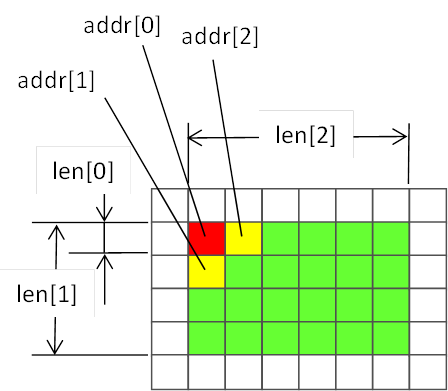
\includegraphics[]{research/sato/fig1.png}
  \caption{Parameters that determines data contiguity}
  \locallabel{fig:fig1}
\end{figure}

\subsubsection{Experimental Results}

\begin{description} 

\item[(1) Himeno benchmark] \ \\

We ported Himeno benchmark program written with MPI to four different CAF programs. They used the same Fujitsu Fortran compiler with the same options including automatic thread parallelization. While the MPI version has 610 lines excluding comment and empty lines, the CAF versions have 402 to 415 lines, 32\% to 34\% shorter.

The result on grid size XL (1024   512   512) is shown in Figure \localref{fig:fig2}. Two CAF programs are respectively 5\% and 2\% faster than the MPI version in average.

\begin{figure}
\centering
  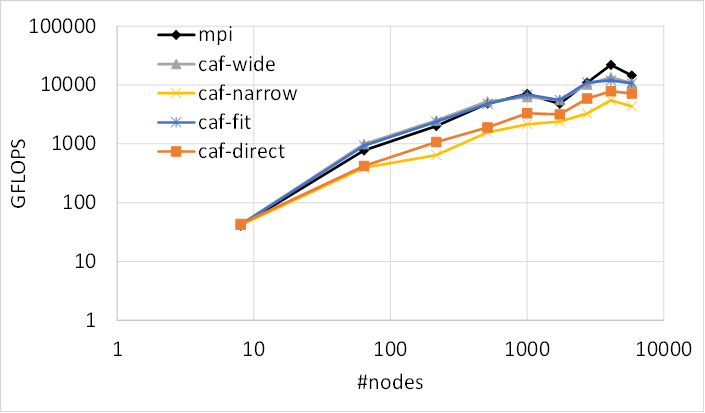
\includegraphics[]{research/sato/fig2.png} 
  \caption
{Four different CAF programs vs. the original MPI on Himeno benchmark}
  \locallabel{fig:fig2}
\end{figure}

\item [ (2) NAS Parallel benchmark ] \ \\

We ported NAS Parallel benchmarks CG, EP, FT and MG written in MPI for CAF respectively. Figure \localref{fig:fig3} shows the result of CG Class-C as an instance and summarizes the history of the CAF program tuning. Finally CAF program V49 exceeds the original MPI version in performance. On EP, the CAF version is only 2\% less performance in average than the original without tuning. On FT, the first version of CAF program extract more than 93\% of the performance of the original in all evaluation ranges of Class B, C and D. Besides the CAF program has still room for performance tuning. On MG, the final version of CAF provides almost the same performance as the original in average.

\begin{figure}
\centering
  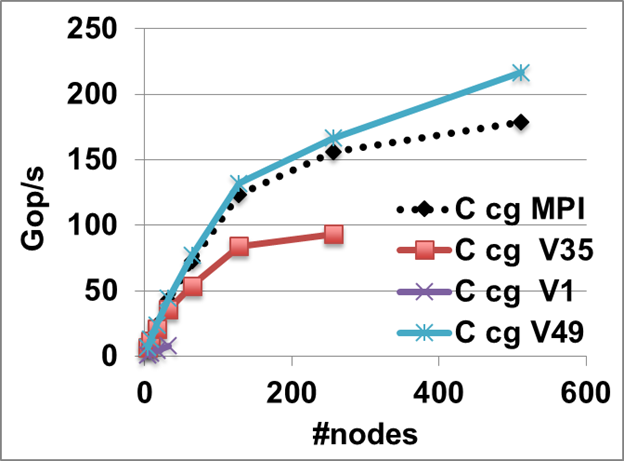
\includegraphics[]{research/sato/fig3.png} 
  \caption {Porting and performance tuning of CAF program on NPB CG Class-C}
  \locallabel{fig:fig3}
\end{figure}

\end{description}

\subsection{ Performance Evaluation of the HPC Challenge Benchmark with XcalableMP}

To evaluate productivity and performance of XcalableMP, we have implemented four benchmarks, namely STREAM, HPL, FFT, RandomAccess, in the HPC Challenge Benchmark Suite by using XcalableMP. 

The figure \localref{fig:fig4} shows that the performance results of the XMP implementations. For a comparison purpose, we have also evaluated the performances of the MPI implementations which are reference implementations. The horizontal axis means that the number of compute nodes, the left vertical axis means that the performance corresponding to the bar, the right vertical axis means that the ratio of the performance of the XMP implementation to that of the MPI implementation corresponding to the line. When the performance ratio is greater than 1, the performance of the XMP implementation is better than that of the MPI implementation. The figure shows that the performances of XMP are almost the same as those of MPI.

\begin{figure}
\centering
  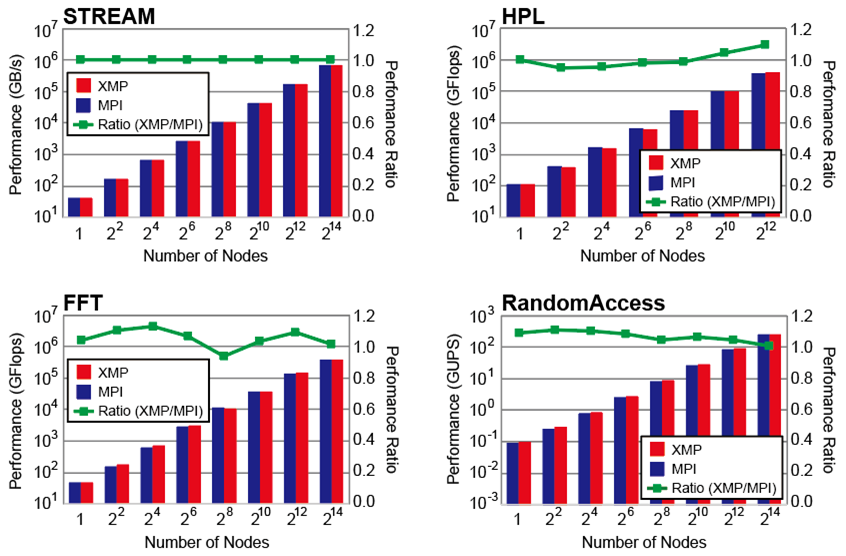
\includegraphics[width=1.0\textwidth]{research/sato/fig4.png}
  \caption{Performance of HPC Challenge Benchmark with XcalableMP}
  \locallabel{fig:fig4}
\end{figure}


The table \localref{tbl:table1}  shows that source lines of code (SLOC) of the benchmarks in XMP and MPI. The table shows that the SLOCs of the XMP implementations are much less than those of the MPI implementations.

\begin{table}
\centering
  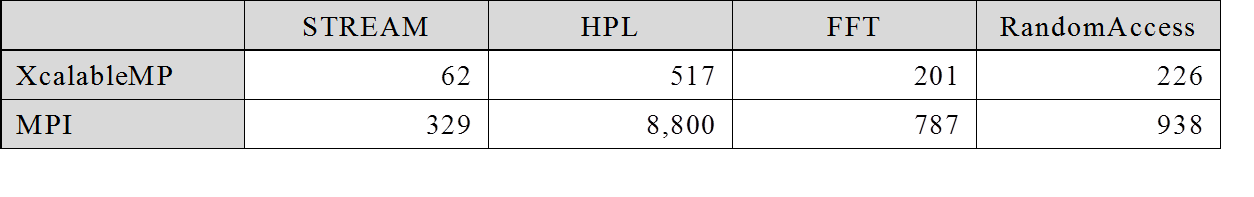
\includegraphics[width=0.9\textwidth]{research/sato/table1.png}
  \caption{SLOC of HPC Challenge Benchmark with XcalableMP}
  \locallabel{tbl:table1}
\end{table}

\subsection { Performance of Three-dimensional Fluid Simulation with XcalableMP
}

The three-dimensional Eulerian fluid code written in Fortran,
IMPACT-3D, which performs compressible and inviscid fluid computation
to simulate converging asymmetric flows related to laser fusion, is
parallelized by three different domain decomposition methods, namely
the domain is divided in (1) only Z direction, (2) both Y and Z
directions and (3) all of X, Y and Z directions using by using
directives only for the “global-view” programming model of
XcalableMP (XMP). The program is also hand-coded with MPI using
the same domain decomposition methods, and the performance difference
between XMP and MPI codes is evaluated on the K computer.

As one node consists of 8 cores in the K computer, one process is
dispatched onto each node and each process performs parallel
computations with 8 threads, which are explicitly described by OpenMP
in both XMP and MPI programs. We run both XMP and MPI codes with three
different decomposition methods and evaluate the weak scaling on the K
computer using Omni XcalableMP/Fortran compiler 0.7.0 and Fujitsu
Fortran K-1.2.0.15. A number of cores for execution and corresponding
simulation parameters are summarized in Table \localref{tbl:table2}. lx, ly, lz are
Fortran array size of first, second, third dimension, and nx, ny, nz
are a number of division in X, Y, Z direction, respectively.

\begin{table}
\centering
  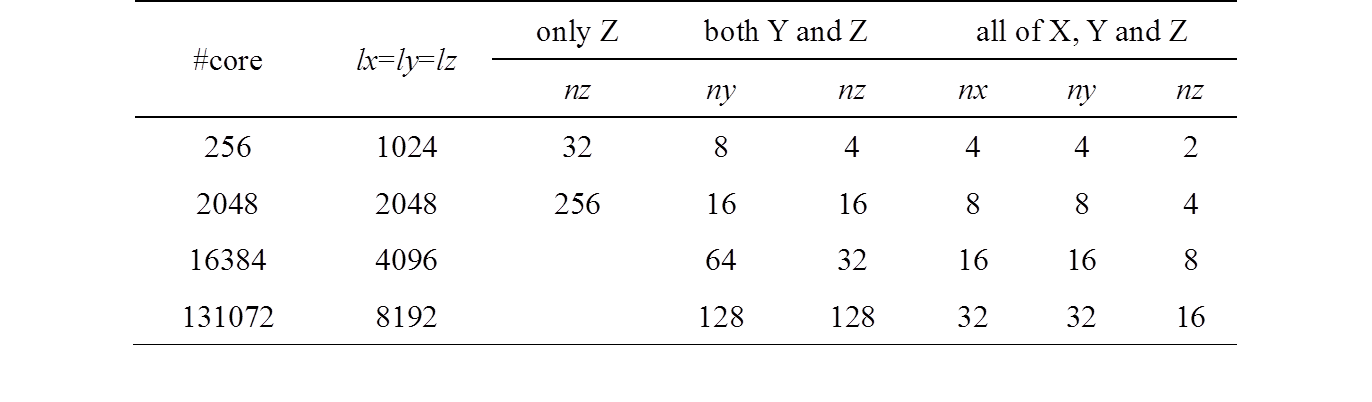
\includegraphics[width=0.9\textwidth]{research/sato/table2.png}
  \caption{Simulation parameters}
  \locallabel{tbl:table2}
\end{table}

Performance is measured by a hardware monitor installed on the K computer, and three indexes are obtained. The total number of floating point operations is counted by the hardware monitor and is interpreted to MFLOPS using elapsed time. Finally it is divided by theoretical peak MFLOPS and output as MFLOPS/PEAK value. The average amount of transfer data per second between memory and CPU is also monitored. It is divided by theoretical peak memory access throughput and output as Memory throughput/PEAK value. The hardware monitor counts the number of instructions, and the number of SIMD instructions is divided by the total number of instructions to obtain SIMD execution usage.

MFLOPS/PEAK values for all 6 cases, namely (MPI, XMP) x (only Z, both Y and Z, all of X, Y and Z) are shown in Fig. \localref{fig:fig5} (a). Performance of XMP codes is as same as that of MPI codes, and small differences among three decomposition methods are found. But we can get only 8 ~ 9 \% of peak performance of the K computer. From the hardware monitor, we found that SIMD execution usage was less than 5\% in all cases, and this could degrade the performance. Most cost intensive DO loops in IMPACT-3D include IF statements, which are needed to correctly treat extremely low velocity and flow direction change regardless of XMP and MPI codes, and the IF statement prevents the native Fortran compiler from generating SIMD instructions inside the DO loop. Thus relatively low performance is obtained.

As the true rate of the IF statement is nearly 100\% in IMPACT-3D, speculative execution of SIMD instruction causes almost no overhead. So forcing the compiler to generate the SIMD instructions could be useful to enhance the performance, and it can be done with “simd=2” compiler option. All codes are recompiled with that option and rerun. SIMD execution usage increases up to around 50\% in all cases, and we can expect performance improvement. MFLOPS/PEAK values for all cases are shown in Fig. \localref{fig:fig5} (b). MPI code performance is improved and we can get up to 20\% of the peak performance. XMP code performance is also improved, but these are below 15\% even XMP code performance is almost same as MPI code performance without “simd=2” option. Although Memory throughput/PEAK values of MPI codes are 55\%, those of XMP codes are only 37\% and this low memory throughput is one of candidates for low sustained performance.

In the converted code by the XMP/F compiler, all Fortran arrays are treated as allocatable arrays even the original code uses static arrays. The allocatable array prevents the native Fortran compiler from optimizing the DO loop with prefetch instructions because the array size cannot be determined at compilation time, and it could cause low memory throughput. All Fortran static arrays in the hand-coded MPI code for the decomposition method of all of X, Y and Z directions are just replaced by allocatable arrays and we check a performance difference. Performance of the MPI code is shown in Fig. \localref{fig:fig5} (c) for static arrays (blue dash) and allocatable arrays (purple dash). MFLOPS/PEAK values are dropped from 20\% to 15\%, and this performance degradation without the prefetch instructions is confirmed. To force the native Fortran compiler to perform the prefetch optimization, we can use additional “prefetch\_stride” compiler option. All codes are recompiled with “simd=2” and “prefetch\_stride” options and rerun. Performance improvements by this compiler option are shown in Fig. \localref{fig:fig5} (c) for both MPI (purple dash to red dash) and XMP (purple solid to red solid) codes. MFLOPS/PEAK values are improved by 2 ~ 3\% with the prefetch optimization.

\begin{figure}
\centering
  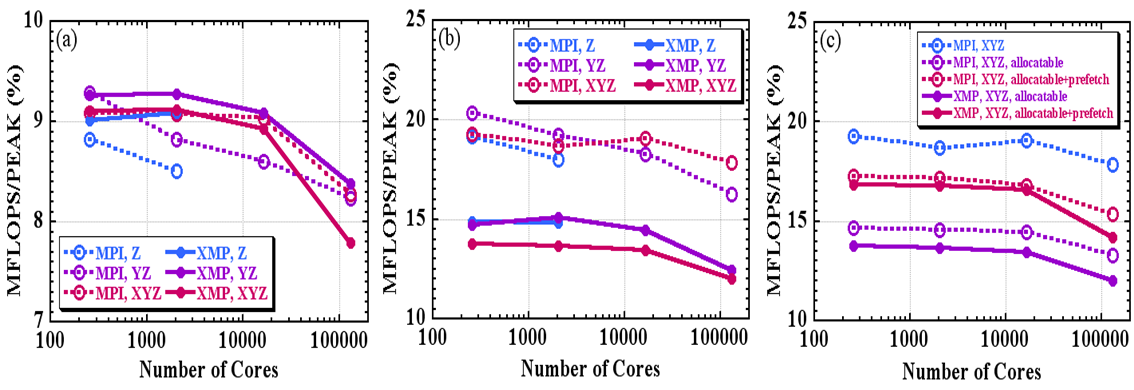
\includegraphics[width=1.0\textwidth]{research/sato/fig5.png}
  \caption{Performance comparison between MPI and XMP on the K computer with (a) no optimization for three decomposition methods, (b) SIMD optimization for three decomposition methods and (c) allocatable array optimization for the decomposition method of all of X, Y and Z directions.}
  \locallabel{fig:fig5}
\end{figure}

\subsection {Design of SCAMP (SCAlable Mpi Profiler) as a co-design tool for large-scale network}

Co-design for HPC is a bidirectional approach, where a system would be designed on demand from applications, and applications must be optimized to the system. In order to co-design the network of large scale systems, it is important to evaluate the communication performance of applications. The trace driven simulator estimates the network performance based on trace files. Firstly, user should run their application on a real system in parallel to obtain the trace files from all processes. These trace files should contain MPI function calls, and their arguments and time stamps, etc. Then, the performance of a virtual system is estimated by using the trace files. While the trace driven simulator is straightforward, sometimes it is not appropriate for the simulation of large parallel systems since it is difficult to obtain the number of trace files for the future system if the current system is smaller than the future one. In order to tackle this scaling-problem in the trace driven simulator, we propose a method called SCAMP (SCAlable Mpi Profiler), which creates a large number of pseudo trace files based on the small number of trace files obtained from a small system and drives the network simulator using the pseudo trace files to estimate the performance of the large systems. 

According to the experiments using SCAMP and using K-computer, as shown in Figure \localref{fig:fig7}, SCAMP overestimates the performance of benchmarks, i.e. the runtime estimated by SCAMP is shorter than the real runtime on K-computer. The reason is that while we have focused only on the network performance, the computation time would change as the number of nodes increases.

\begin{figure}
\centering
  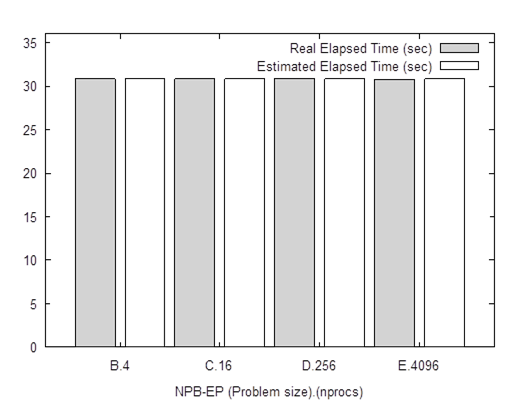
\includegraphics[width=0.45\textwidth]{research/sato/fig6.png}
  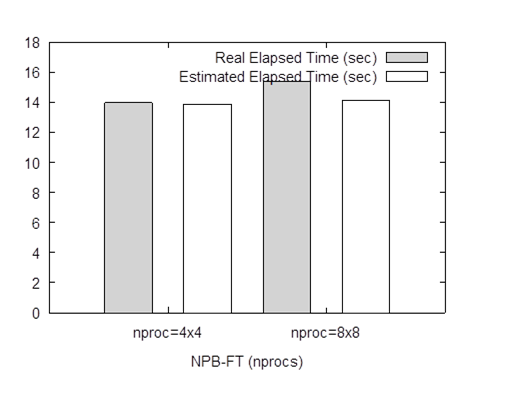
\includegraphics[width=0.5\textwidth]{research/sato/fig7.png}
  \caption{Comparison between real time and estimated time by SCAMP}
  \locallabel{fig:fig7}
\end{figure}

\subsection{Performance evaluation of Tascell on the K computer}
 
Tascell is a task parallel language that supports distributed memory environments. A Tascell worker spawns a real task only when requested by another idle worker. The worker spawns a task after restoring its oldest task-spawnable state by temporarily backtracking. This mechanism eliminates the cost of spawning/managing logical threads. It also promotes the reuse of workspaces and improves the locality of reference since it does not need to prepare a workspace for each concurrently runnable logical thread. Furthermore, a single Tascell program can run efficiently on shared and distributed memory environments.

This study aims to evaluate Tascell on massively parallel systems; in particular, we employed 1024 nodes of the K Computer with 8192 cores in total. In addition, we revised the implementation of Tascell to get it working on such systems.

In the conventional implementation of Tascell, inter-node communication is realized by TCP/IP communication via message routing servers called Tascell servers. This implementation is suitable for dynamic addition of computation nodes and wide-area distributed environments. On the other hand, Tascell servers often become communication bottlenecks. Furthermore, in recent supercomputer environments, there may be no appropriate places for deploying Tascell servers, and TCP/IP may not be available for inter-node communication; it is hard or impossible to run the conventional implementation in such an environments.

Therefore, we implemented inter-node communication in Tascell using MPI, which is supported by most practical supercomputer systems. At the same time, we adopted a server-less implementation in order to overcome the deployment and bottleneck problems, excluding the support of wide-area distributed environments. Note that programmers can write Tascell programs without concern about the underlying communication layer.

We evaluate the performance of our MPI-based implementation on the K computer using 7168 workers (7 workers x 1024 nodes).
The result is shown in Figure \localref{fig:fig8}.

In order to enable our implementation to work with the MPI implementation on the K computer and many other MPI implementations, it only requires the MPI\_THREAD\_FUNNELED support level, in which only the main thread can make MPI calls, and the two-sided communication paradigm. With such minimum requirements, our MPI-based implementation successfully realized both high performance and deadlock freedom.

\begin{figure}
\centering
  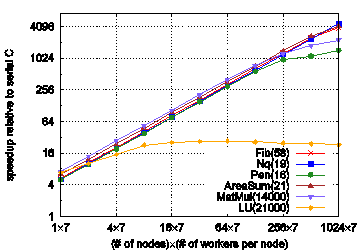
\includegraphics[width=0.9\textwidth]{research/sato/fig8.png}
  \caption{Evaluation results (Speedup) of Tascell programs on the K computer}
  \locallabel{fig:fig8}
\end{figure}

\section{Schedule and Future Plan}

From this year, we started the study of the programming models for post-petascale, including programming models and runtime techniques to support manycore. We already propose XcableACC as a solution for accelerator-based system, which is to be explored in the JST CREST project. As the post-K computer will be a large-scale multicore-based system, we will investigate programming models for manycore-based parallel systems including dynamic tasking and load balancing as well as advanced PGAS models for distributed memory systems.

As in recent years, an important action for XcalableMP project is to disseminate our XcalableMP to applications users. As in last years, we organized several schools and hands-on, workshop with potential users also in this year. We will continue these promotion activities while we will study more optimization technique of XcalableMP compiler to improve the performance. As a research agenda especially for the K computer, we will contribute the scalability of large-scale applications for the K computer.

%%% DO NOT EDIT BELOW

\section{Publications}

%\printbibliography[keyword=journal, heading=subbibliography, title={Journal Articles}, prefixnumbers={1-}, resetnumbers=true]
%\printbibliography[keyword=proceedings, heading=subbibliography, title={Conference Papers}, prefixnumbers={2-}, resetnumbers=true]
%\printbibliography[keyword=invited, heading=subbibliography, title={Invited Talks}, prefixnumbers={3-}, resetnumbers=true]
%\printbibliography[keyword=poster, heading=subbibliography, title={Posters and Presentations}, prefixnumbers={4-}, resetnumbers=true]
%\printbibliography[keyword=deliverable, heading=subbibliography, title={Patents and Deliverables}, prefixnumbers={5-}, resetnumbers=true]

\printbibliography[keyword=journal, heading=subbibliography, title={Journal Articles}, resetnumbers=true]
\printbibliography[keyword=proceedings, heading=subbibliography, title={Conference Papers}]
\printbibliography[keyword=invited, heading=subbibliography, title={Invited Talks}]
\printbibliography[keyword=poster, heading=subbibliography, title={Posters and Presentations}]
\printbibliography[keyword=deliverable, heading=subbibliography, title={Patents and Deliverables}]

\end{refsection}
